\documentclass[11pt, oneside]{article}   	% use "amsart" instead of "article" for AMSLaTeX format
\usepackage{geometry}                		% See geometry.pdf to learn the layout options. There are lots.
\geometry{letterpaper}                   		% ... or a4paper or a5paper or ... 
%\geometry{landscape}                		% Activate for rotated page geometry
\usepackage[parfill]{parskip}    		% Activate to begin paragraphs with an empty line rather than an indent
\usepackage{graphicx}				% Use pdf, png, jpg, or eps§ with pdflatex; use eps in DVI mode
								% TeX will automatically convert eps --> pdf in pdflatex		
\usepackage{amssymb}

%SetFonts

%SetFonts
\usepackage{listings}
\usepackage{color}

\definecolor{dkgreen}{rgb}{0,0.6,0}
\definecolor{gray}{rgb}{0.5,0.5,0.5}
\definecolor{mauve}{rgb}{0.58,0,0.82}

\lstset{frame=tb,
  language=c++,
  aboveskip=3mm,
  belowskip=3mm,
  showstringspaces=false,
  columns=flexible,
  basicstyle={\small\ttfamily},
  numbers=none,
  numberstyle=\tiny\color{gray},
  keywordstyle=\color{blue},
  commentstyle=\color{dkgreen},
  stringstyle=\color{mauve},
  breaklines=true,
  breakatwhitespace=true,
  tabsize=3
}


\title{ImSecu Lab : Watermarking and Biometrics}
\author{Antoine PELLETIER}
\date{}							% Activate to display a given date or no date

\begin{document}
\maketitle
\tableofcontents
\newpage
\section{Least Significant Bit}
	\subsection{Code and results}
In this first section, we are going to watermark an image by tampering the Least Significant Bit (LSB) of each component (RGB) of each pixel. The tampering will be a pseudo random noise. The first function we have to complete is InsertNoiseLSB. 
\begin{lstlisting}
int CImage::InsertNoiseLSB(){
	int noise;
	srand(0);
	noise=rand()%2;
	for (int c=0; c<nb_comp;c++) {//For each component
		if (C[c]==NULL)
			return ERROR;		
		else
			for(int i=0;i<width;i++){        //For all
				for(int j=0;j<height;j++){// the pixels,
					SETBIT(C[c][i+j*width],0,noise); /*Set the pixel LSB value to randomly 0 or 1*/
					noise=rand()%2; /*Change the random value*/
				}
			}
	}
	return SUCCESS;
}
\end{lstlisting}
\newpage
Then, to test if an watermarked image has been tampered, we are going to check, for each component of each pixel, the value of the LSB and compare it with the pseudo random value expected. As we use the same seed for watermarking and testing, we will get the same pseudo random sequence. Here is the completed code of the ExtractNoiseLSB function.
\newline
\begin{lstlisting}
int CImage::ExtractNoiseLSB(){
	int noise;
	srand(0);
	int LSBValue;

	for (int c=0; c<nb_comp;c++) {// For each component
		if (C[c]==NULL)
			return ERROR;	
		else
			for(int i=0;i<width;i++){        //For all 
				for(int j=0;j<height;j++){// the pixels
					noise=rand()%2;//Calculate the expected value of the LSB
					LSBValue=GETBIT(C[c][i+j*width],0);//Get the actual value of the LSB
					if(LSBValue==noise){//If the two values are the same,
						C[c][i+j*width]=0;//Set the component value to 0
					}
					else{
						C[c][i+j*width]=255;//If they are equal, set the component value to 255
					}
				}
			}
	}      
	return SUCCESS;
}
\end{lstlisting}
Now we will watermark an image of a lezard. Then we will check the integrity of the watermarked image. The result is the following.
\newpage
			\begin{figure}[h]
			\begin{center}
				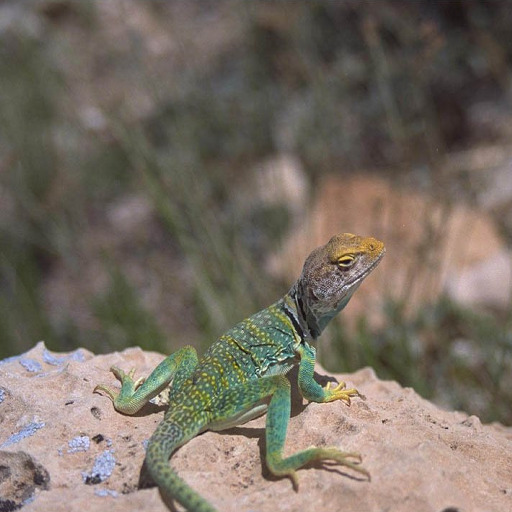
\includegraphics[scale=0.35]{images_png/image3.jpg}
				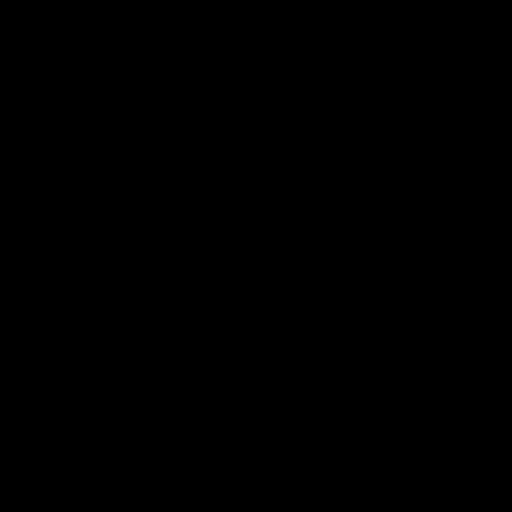
\includegraphics[scale=0.35]{images_png/image5.jpg}
			\end{center}
			\caption{Watermarked image of a lezard (left) and the check of this image (right)}
			\end{figure}
		
			As we can see, the checked image is all black. It's normal because as the image hasn't been tamper, all the component values has been set 0 and in RGB, (0,0,0) is black.
			\newline
			Now we are going to tamper the watermarked image by changing the hue, contrast and saturation value of some areas. Then we are going to check the result of the check on this tampered image. The result are the following.	
			\begin{figure}[h]
			\begin{center}
				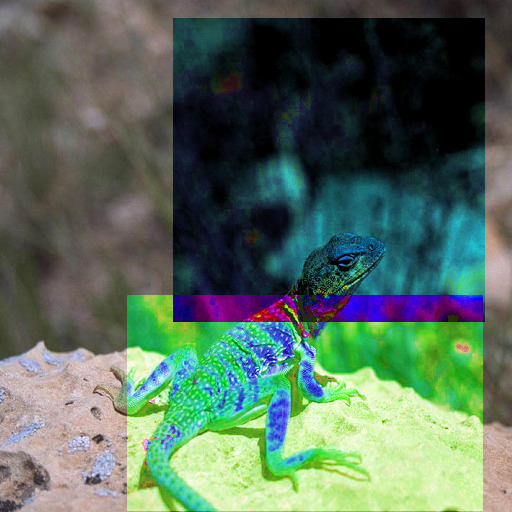
\includegraphics[scale=0.342]{images_png/image6.jpg}
				
\includegraphics[scale=0.342]{images_png/image7.jpg}
			\end{center}
			\caption{Tampered image of a lezard (left) and the check of this image (right)}
			\end{figure}
	
			As we can see, the tampered areas are well detected. 
\subsection{Questions}
As showed previously, this method of putting random noise in the LSB allow to detect the tampered zone of an image. However, even if the areas are strongly tampered, the check isn't white. Some component's LSB haven't been changed (else the area would be all white). 
\newline
We can obtain white zone by slightly modifying the luminosity of an area. This result is counter intuitive because we will expect the more tampered zone to be "more" white (ie detected). However, this method only change the LSB of each pixel. It is possible that tampering is huge and does not change the LSB (that is why the high tampered zone on the previous example is not all white). \newline On the opposite, small changes can heavily modify the LSB. \newline
The PSNR of this technique is pretty high, it is calculated as follows :
\begin{lstlisting}
MSE=average([original(x,y)-watermarked(x,y)]^2)
MAX=255
PNSR=10*10log10(max^2/MSE)
\end{lstlisting}
As the noise affect the LSB of the image, MSE is small and the PSNR is high. So this method provide a good visibility, which is a good point.
\newline
A bad point is that this method is not really reliable. Indeed, if we can tamper only the most significant bits of the image, the apparence would be completely different but this method won't detect the changes. Moreover, this method is independent of the image, so once the watermarking procedure is known, it can be easily counterfeited and therefore can not be used for authentication.
\section{Least Significant Bit and Cyclic Redundancy Check}
\subsection{Code and results}
Now we are going to implement a way to allow authentication by making the protection data dependent. To do so the image will be divided in blocks and we will compute a checksum of the Most Significant Bit (MSB) of each block and hide this checksum in the LSB of the pixels of the block. First we need to complete the function to insert the checksum in the block. \newline
\begin{lstlisting}
int CImage::InsertCRCLSB(){
	int nb_xblocks = width/8;
	int nb_yblocks = height/8;
	unsigned long crc;
	unsigned long *crcTable;
	short bit;
	
	CRCTable(&crcTable);

	for (int c=0; c<nb_comp;c++) {
		if (C[c]==NULL)
			return ERROR;	
		for (int i=0; i<nb_xblocks; i++)
			for (int j=0; j<nb_yblocks; j++) {
				/* A COMPLETER */
				crc = CRCBlock(c,8*i,8*j,8,8,crcTable);//Compute the checksum of the block (i,j)
					for (int k=0; k<32; k++){
					bit=GETBIT(crc,k);//Get the k-th bit of crc
					SETBIT(									//Set
						C[c][8*i+k%8+width*(8*j+k/8)],  //the corresponding pixels
						0,									//LSB
						bit									//to bit
					);	
					}
			}
	}
	free(crcTable);
	return SUCCESS;
}
\end{lstlisting}
When we have the checksum, we insert it in the LSB of the 32 first pixels of block \((i,j)\). The upper right pixel of the block \((i,j)\) can be access by \(C[c][8*i+width*(8*j)]\). The 8 first bits of the blocks are access simply by adding 1 to this (this is the role of the \(k\%8)\). It is a bit more complex to jump to the second line of the block. We need to add \(width*k/8\) to jump to the \(k/8\) line of the block. Note that in C++, \(k/8\) is an integer !\newline At the end we get the final expression to access the 32 first bits of the blocks : \newline \[C[c][8*i+k\%8+width*(8*j+k/8)] \]
\newpage
Now that we are able to insert a CRC in an image, we also need to be able to extract it. So we complete the following function.
\begin{lstlisting}
int CImage::ExtractCRCLSB(){
	int nb_xblocks = width/8;
	int nb_yblocks = height/8;
	unsigned long crc, xcrc;
	unsigned long *crcTable;
	short bit;

	CRCTable(&crcTable);	
	
	for (int c=0; c<nb_comp;c++) {
		if (C[c]==NULL)
			return ERROR;	
		for (int i=0; i<nb_xblocks; i++)
			for (int j=0; j<nb_yblocks; j++) {	
			/* A COMPLETER */
				crc = CRCBlock(c,8*i,8*j,8,8,crcTable);//Compute the checksum of the block (i,j)
				for (int k=0; k<32; k++){
					bit=GETBIT(C[c][8*i+k%8+width*(8*j+k/8)],0)//Get the LSB of the 32 first pixels
					SETBIT(xcrc,k,bit);//And put them in xcrc
				}
				if(crc!=xcrc){// If the value is different of the expected one
					DrawBadBlock(8*i,8*j,8,8); // Draw a bad block
				}
			}
	}
	free(crcTable);
	return SUCCESS;
}
\end{lstlisting}
Here is what we get when watermarking an image, tampering it and checking it. \newpage
			\begin{figure}[h]
			\begin{center}
				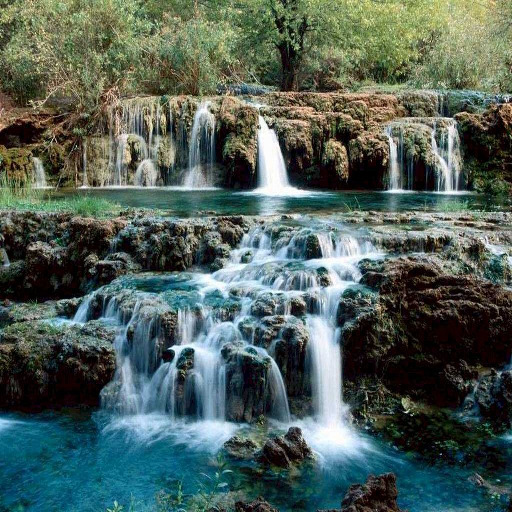
\includegraphics[scale=0.34]{images_png/image0.jpg}
				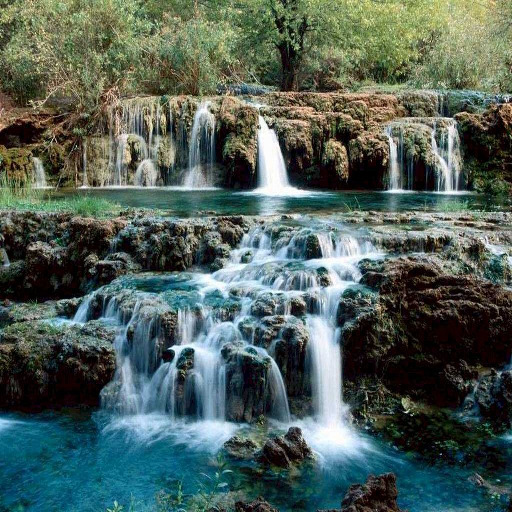
\includegraphics[scale=0.34]{images_png/image0.jpg}
			\end{center}
			\caption{Original image of a cascade (left) and the watermarking of this image (right)}
			\end{figure}
			\begin{figure}[h!]
			\begin{center}
				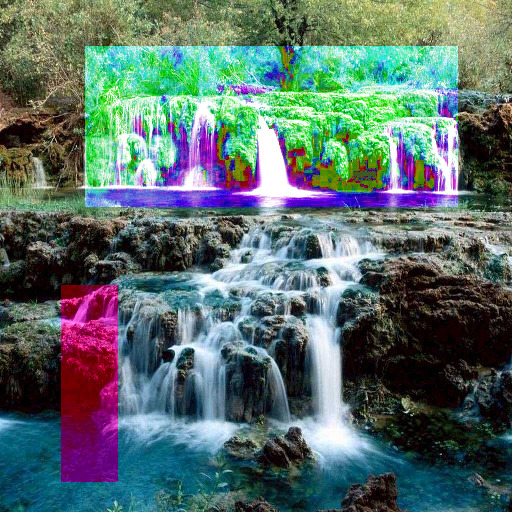
\includegraphics[scale=0.34]{images_png/image1.jpg}
				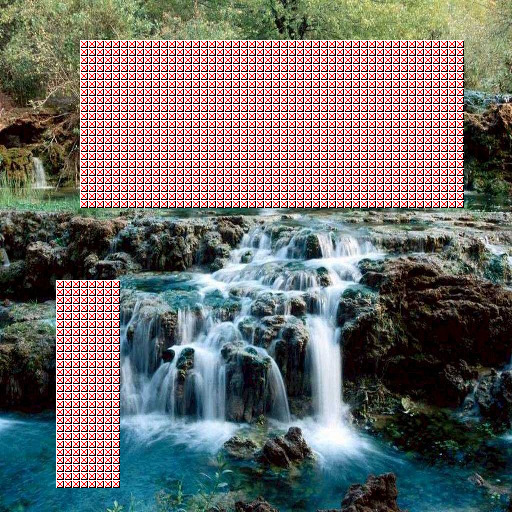
\includegraphics[scale=0.34]{images_png/image2.jpg}
			\end{center}
			\caption{Tampered image of a cascade (left) and the check of this image (right)}
			\end{figure}
\subsection{Questions}
As before, we can see that the watermarking preserves the visibility. The noise is still added to the LSB. Moreover, there are twice less pixels modified compared with the first method. So the PSNR is lower or equal. \newline In term of reliability, this method is more efficient than the precedent. Indeed, to pass the check, the checksum of the block has to remain unchanged, and not only the LSB as before. Moreover, if an attacker want to tamper a watermarked image, the checksum has to remain unchanged for all the component ! \newline
In the CRCBlock function, before calculating the CRC of a block, the LSB of the pixel is set to 0 like this :
\begin{lstlisting}
			val = (int)C[c][posx+k + (posy+l)*width];
			SETBIT(val,0,0);
\end{lstlisting}
The reason is simple. We need to calculate two times the CRC of a block : to watermark an image and to check it. And the difference between an watermarked image and the original image is only in the 32 first pixels LSB of each block. In order to have the same CRC for each block between the original image and the watermarked-but-not-tampered one, we need to discard the LSB of the calculus of the CRC.
\section{Least Significant Bit, Cyclic Redundancy Check and Self-Embedding}
\subsection{Code and results}
In this last part, we will implement the same as before but we will add a recovery process for the tampered area. First we complete the BlockMean function which will be used for getting the mean of a block. 
\begin{lstlisting}
nt CImage::BlockMean(short *value, int c, int posx, int posy,
							 int block_width, int block_height){

	if (C[c]==NULL)
		return ERROR;
	if (posx<0 || posy<0 || posx+block_width-1>width
		 ||posy+block_height-1>height)
		return ERROR;
	/* A COMPLETER */
	long int sum=0;
	int x,y;
	for (x=posx;x<posx+block_width;x++){ //For each pixel of the block
		for (y=posy;y<posy+block_height;y++){
			sum+=C[c][x+width*y]; // add its value to the sum
		}
	}
	(*value) = (short)(sum/(block_width*block_height)); //divide by the number of pixels to get the mean
	return SUCCESS;
}
\end{lstlisting}
Now we complete the watermarking function, ie InsertSelfLSB.
\begin{lstlisting}
int CImage::InsertSelfEmbeddingLSB(){
	int nb_xblocks = width/8;
	int nb_yblocks = height/8;
	unsigned long crc;
	unsigned long *crcTable;
	short bit;
	short m[4];
	int ti,tj;
	CRCTable(&crcTable);
	ti = 4;
	tj = 4;
	for (int c=0; c<nb_comp;c++) {
		if (C[c]==NULL)
			return ERROR;	
		for (int i=0; i<nb_xblocks; i++){
			for (int j=0; j<nb_yblocks; j++) {
				/* A COMPLETER */
				crc = CRCBlock(c,8*i,8*j,8,8,crcTable);//Compute the checksum of the block (i,j)
				for (int k=0; k<32; k++){
					bit=GETBIT(crc,k);//Get the k-th bit of crc
					SETBIT(									//Set
						C[c][8*i+k%8+width*(8*j+k/8)],  //the pixel's at posx=(8*i+k%8) and posy=(8*j+k/8)
						0,									//LSB
						bit									//to bit
					);	
				}
				//Compute the mean of the 4 blocks
				BlockMean(&m[0],c,i*8     ,j*8	,4,4);
				BlockMean(&m[1],c,i*8+4,j*8	   ,4,4);
				BlockMean(&m[2],c,i*8     ,j*8+4,4,4);
				BlockMean(&m[3],c,i*8+4,j*8+4,4,4);
				//Set the last 32 LSB according to mean
				for(int k=0;k<4;k++){//for each sub-block
					for(int l=0;l<8;l++){//for each bit
						bit=GETBIT(m[k],l);
						SETBIT(C[c][ ((8*(i+ti)+l)%width) +width* ((8*(j+tj)+k+4)%height) ],0,bit);
					}
				}
			}
		}
	}
	free(crcTable);
	return SUCCESS;
}
\end{lstlisting}
Finally, we complete the last function, which is the check and restore function.
\begin{lstlisting}
int CImage::ExtractSelfEmbeddingLSB(){
	int nb_xblocks = width/8;
	int nb_yblocks = height/8;
	unsigned long crc, xcrc=0;
	unsigned long *crcTable;
	short bit;
	short m[4];
	int ti,tj;
	CRCTable(&crcTable);
	ti = 4;
	tj = 4;
	for (int c=0; c<nb_comp;c++) {
		if (C[c]==NULL)
			return ERROR;	
		for (int i=0; i<nb_xblocks; i++)
			for (int j=0; j<nb_yblocks; j++) {
				/* A COMPLETER */
				crc = CRCBlock(c,8*i,8*j,8,8,crcTable);//Compute the checksum of the block (i,j)
				for (int k=0; k<32; k++){
					bit=(short)GETBIT(C[c][8*i+k%8+width*(8*j+k/8)],0);
					SETBIT(xcrc,k,bit);
				}//Get the checksum embeded in the block
				if(crc!=xcrc){//if this is not a match,
					//extract the restoration bits
					m[0]=0;// don't know why 
					m[1]=0;// but we get an error
					m[2]=0;// if those value are not
					m[3]=0;// initialized 	
					for(int k=0;k<8;k++){//for each sub-block
						for(int l=0;l<4;l++){//for each bit
							bit=(short)GETBIT(C[c][ (8*(i+ti)%nb_xblocks+k) +width* (8*(j+tj)%nb_yblocks+l+4) ],0);//get the value to restore
							SETBIT(m[l],k,bit); // and save it in m[l]
						}
					}
					
					//Restoration of the tampered blocks
					DrawFlatBlock(c,8*i  ,8*j  ,4,4,m[0]);
					DrawFlatBlock(c,8*i+4,8*j  ,4,4,m[1]);
					DrawFlatBlock(c,8*i  ,8*j+4,4,4,m[2]);
					DrawFlatBlock(c,8*i+4,8*j+4,4,4,m[3]);
				}
			}
		}
	free(crcTable);
	return SUCCESS;
}
\end{lstlisting}
Here is what we get when testing this new watermarking method on an image.
			\begin{figure}[h!]
			\begin{center}
				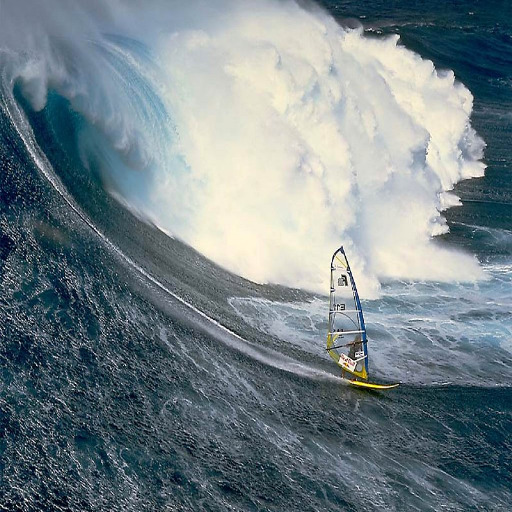
\includegraphics[scale=0.34]{images_png/image8.jpg}
				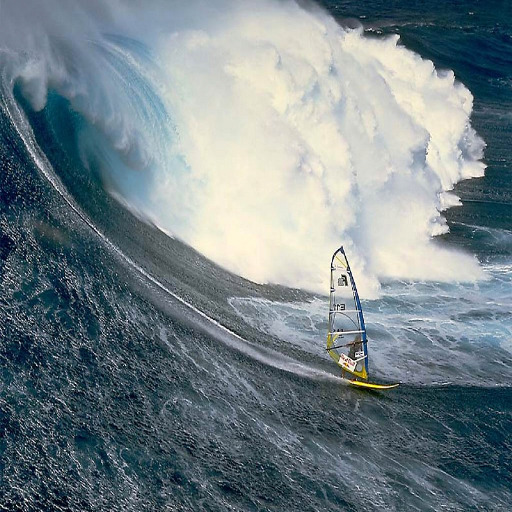
\includegraphics[scale=0.34]{images_png/image9.jpg}
			\end{center}
			\caption{Original image of a wave (left) and the same image watermarked (right)}
			\end{figure}
			\newline
			As expected, the watermark preserves the visibility of the image. Regarding the PSNR, we can assume that it is comparable to the second technique and less than the first one that is pseudo random noise.
			\begin{figure}[h!]
			\begin{center}
				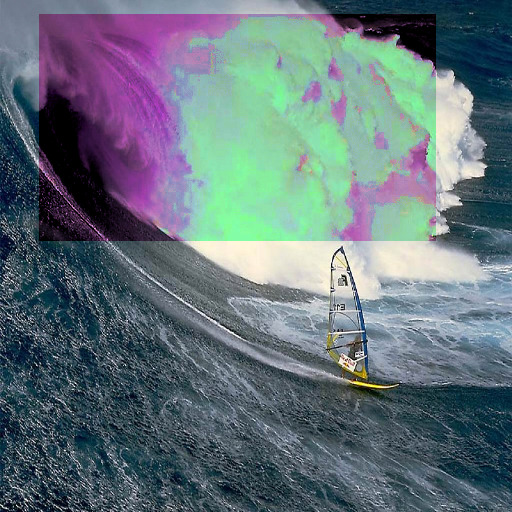
\includegraphics[scale=0.34]{images_png/image10.jpg}
				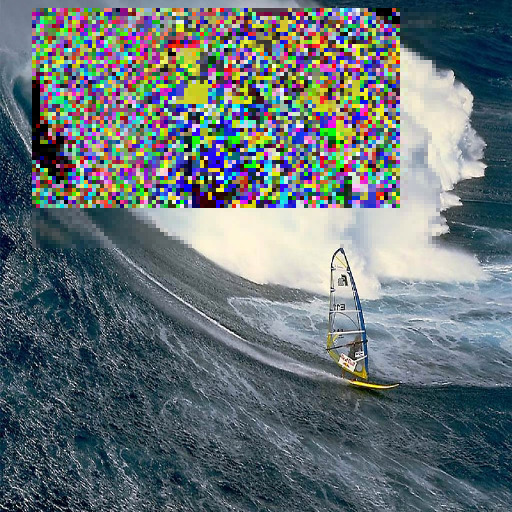
\includegraphics[scale=0.34]{images_png/image11.jpg}
			\end{center}
			\caption{Tampered image of a wave (left) and the check of this image (right)}
			\end{figure}
			\newpage
\subsection{Questions}
The reconstruction did not work completely. It was predictable because the reconstruction block are not distant enough regarding the size of the tempered area. Indeed, as the translation is \((4,4)\), the maximum reconstructible area is a band of height or width of 4 blocks. \newline
Here we can see that the bottom and right border of the tampered zone has been successfully rebuilt. The reason is that their restoration blocks were not tampered, whereas the other region of the tamper area could not be restored because their restoration blocks has been altered. This illustrate the necessity to embed the restoration bits in a distant block.\newline
As explained earlier, the limitation of the restoration functionality is the size of the tempered zone. Moreover, it is clear that even when the restoration bits were not altered, the reconstruction is pixelated due to the flat block reconstruction.
\section{Comparison of the three methods}
The three methods presented in this labs have some common point, due to the fact that we mainly watermark using the LSB. \newline As a consequence, all those techniques offers a good visibility with a high PSNR. With the random noise and self-embedding methods, all the pixels LSB are modified whereas with CRC, only half of the pixels LSB are altered. \newline
In term of reliability, the first method is the worst because the 7 most significant bit of each pixel can be modified without being detected. For the two other methods, the reliability is better thanks to the use of the CRC, which prevent tampering without a lost of visibility. \newline
The complexity increased across the methods. The first one has a low level complexity because it is done pixel by pixel and the verification is easy and does not require more than a random generator. The second methods is more complex due to the abstraction of blocks and the computation of CRC. The last method is the most complex because it uses CRC as the previous one and also add the complexity of dealing with the restoration bits. \newline
The first method offers a pixel by pixel tampering detection, the second method a block tampering detection, and the last method offers a block tampering detection and a reconstruction functionality. However, this last functionality is not really fully efficient due to some obvious limitations discussed earlier.
\newline
\newline
A common drawback to all those methods is that the watermarking isn't reversible and causes a loss of information. Indeed, we lost a eighth of the information because we use the LSB to watermark. Moreover, if an image is compressed, all those methods would consider it as a tampering. As a consequence, the major drawback shared by all those methods is their sensitivity: they will consider almost everything as tampering (slight light shift, compression, color balancing etc) and could miss some obvious (visible) tampering. For example, the modification of the 7 MSB with the first method would be undetected. 
\end{document}